\section{Mobiliteitsvraagstuk}
De auto is het slachtoffer geworden van zijn eigen succes: we staan meer dan ooit in de file en de CO2 van personenverkeer stijgt jaar na jaar. De belg neemt al snel de auto voor korte afstanden ($<$ 25 km). In deze auto zit meestal maar 1 persoon. Het Belgische wagenpark blijft groeien (figuur \ref{fig:wagenpark}). Hier zien we wel een trend ontstaan. Er worden steeds meer elektrische en hybride wagens verkocht, maar die staan natuurlijk net zo goed in de file. Mobiliteit op twee wielen kan hier een oplossing bieden.
\\

\begin{wrapfigure}{R}{0.40\textwidth}
  \centering
  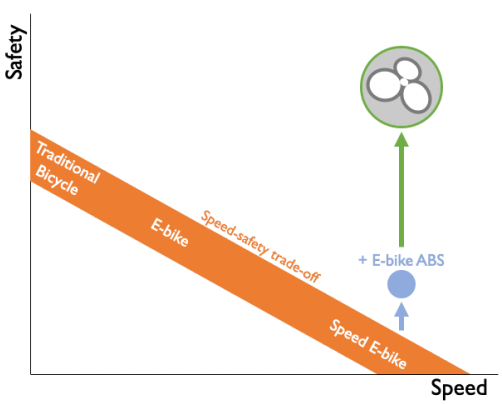
\includegraphics[width=1.1\linewidth]{images/snelheid-veiligheid-tradeoff.png}
  \caption{Snelheid-veiligheid trade-off (bron: IntuEdrive)}
  \label{fig:snelheid-veiligheid trade-off (bron: IntuEdrive)}
\end{wrapfigure}

Mobiliteit op twee wielen kennen we al lang: fietsen bestaan al sinds de 19de eeuw. Elektrische fietsen hebben het potentieel van deze tweewielers enorm verhoogd: fietsen wordt moeiteloos en stukken sneller. Spijtig genoeg neemt het risico op ongevallen ook toe bij hogere snelheid. Dat komt omdat e-bikes en speed e-bikes precies dezelfde technologie gebruiken als normale fietsen – grote wielen met smalle banden, kettingaandrijving met manuele versnellingen, mechanische handremmen – bij veel hogere snelheden. IntuEdrive noemt dit de snelheid-veiligheid trade-off. De veiligheid kan beperkt worden verhoogd door componenten toe te voegen (bv. Bosch e-bike ABS), maar de functionaliteit van deze systemen blijft beperkt. Er is een meer holistische aanpak nodig. Bovendien bieden elektrische fietsen vandaag nog niet het gebruiksgemak en de betrouwbaarheid die de consument gewend is van zijn wagen.
\\\\
IntuEdrive’s \textit{CoSaR} is een snelle elektrische fiets die veiliger is dan de klassieke mechanische fiets, dankzij hun innovatie tweewielaandrijving en elektrische remfunctie. Dit systeem reduceert de stopafstand met 60\% en maakt schakelen overbodig (automatische versnellingen). Het stapt ook af van de onderhoudsintensieve fietscomponenten (ketting, tandwielen, mechanische remmen). Dit maakt CoSaR de perfecte e-bike voor woon-werkverkeer: makkelijk, veilig en betrouwbaar.
\\\\
Door automatisch te schakelen zorgt CoSaR ervoor dat de fietser in elke situatie precies zo snel trapt als hij of zij wil. Deze gewenste trapsnelheid – of beter trapcadans – varieert van persoon tot persoon en hangt af van omstandigheden zoals helling, tegenwind en rijsnelheid. Omdat deze gewenste cadans niet op voorhand gekend is, schakelt de transmissie momenteel op basis van een vaste wetmatigheid die tijdens testen getuned is om voor zoveel mogelijk gebruikers comfortabel aan te voelen. Wijkt deze wetmatigheid af van de gewenste cadans van een specifieke gebruiker, dan kan deze gebruiker via knoppen op het stuur tijdens het fietsen zijn of haar cadans manueel aanpassen.
\\
\begin{figure}
  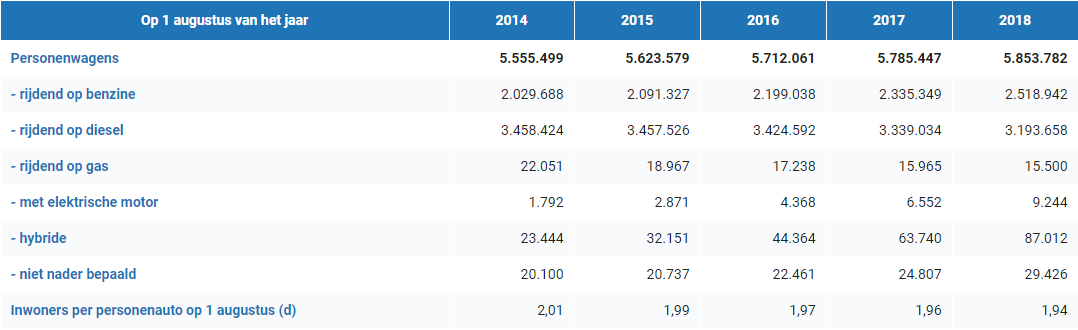
\includegraphics[width=\linewidth]{images/wagenpark_belgie.png}
  \caption{Grootte van het voertuigenpark 2014-2018 (bron: statbel.fgov.be)}
  \label{fig:wagenpark}
\end{figure}


\section{Online machine learning voor geïndividualiseerde cadanscontrole}
Deze thesis werkt verder op het prototype geleverd door IntuEdrive. Zoals reeds aangehaald schakelt de fiets automatisch. De trapcadans wordt hierdoor stabiel gehouden, ook wanneer de fietser harder of zachter trapt. Het doel is om deze instelling te veranderen door de cadans van de e-bike in real time te voorspellen aan de hand van de toestand van de fiets, zodat de trapsnelheid zich aanpast aan de huidige omstandigheden en de individuele gebruiker. Deze implementatie zal ervoor zorgen dat de fietser meer aandacht kan besteden aan de weg, waardoor gevaarlijke situaties kunnen vermeden worden. Om de cadans te personaliseren en dynamisch te maken, zal een machine learning algoritme ontwikkeld worden dat de toestand van de fiets als input binnenkrijgt en hiermee de trapsnelheid berekent. Wanneer de fietser besluit om de cadans manueel aan te passen, interpreteert het algoritme dit als een signaal om bij te leren.
\\\\
Om de performantie van het machine learning algoritme te testen zal het volledig systeem fiets-fietser-cadanscontrole gesimuleerd worden. Het fietsmodel wordt geleverd door IntuEdrive en zal geïmplementeerd worden in python. Vervolgens worden een aantal machine learning algoritmes vergeleken op basis van een aantal vooraf gedefinieerde performance indicatoren. De machine learning algoritmes zijn afkomstig uit scikit-learn, een machine learning library.
\\\\
De cadanscontrole moet aan verschillende eisen voldoen. Het algoritme moet draaien op een Raspberry Pi, samen met het controleprogramma van de fiets. Door deze beperkte resources moet het algoritme zo efficiënt mogelijk zijn. De voorspellingen moeten bijna in real time berekend worden. Het doel is om aan 10Hz de cadans aan te passen, maar hoe meer voorspellingen per seconde, hoe beter. Tragere voorspellingen kunnen hinderlijk zijn voor het rijgedrag. Ten slotte moet er ook rekening gehouden worden met de veiligheid van de fietser. Opeenvolgende voorspellingen mogen niet te veel van elkaar verschillen, anders zou de fietser erdoor gestoord kunnen worden en zijn concentratie verliezen. Bovendien mag de cadans nooit hoger dan een bepaalde maximum limiet ingesteld worden.
\\\\
De algoritmes worden geëvalueerd op basis van de mean squared error tussen de ingestelde cadans - afkomstig van het machine learning algoritme - en de zogenaamde \textit{\gls{fcc}} van de fietser. Die freely chosen cadence is niet precies gekend en wordt in de simulatie bepaald aan de hand van een fietsersmodel. Dit is een functie die de toestand van de fiets en de fietser (rijsnelheid, helling,...) afbeeldt op de trapsnelheid die de fietser in dat geval het meest comfortabel vindt. Simpel gezegd is het fietsersmodel een functie met als input de toestand van de fiets en als output een “optimale cadans”. Deze functie is speculatief en kan makkelijk aangepast worden. Op welke basis de fietser precies zijn freely chosen cadence bepaalt is voor dit onderzoek weinig relevant. Het gaat er hier vooral om dat het machine learning algoritme het fietsersmodel kan achterhalen.
\\
\begin{center}
Fietsersmodel:\tab fcc = f(snelheid,koppel,vermogen,helling,...)
\end{center}
Het algoritme moet kunnen bijleren met een kleine hoeveelheid data. De gebruiker zal immers niet vaak manuele aanpassingen doen aan de cadans. Te veel data gebruiken kan een negatieve invloed hebben op reeds correcte voorspellingen. Het algoritme moet ook snel bijleren. Elke verandering moet zo snel mogelijk doorgevoerd worden en moeten een betekenisvolle impact hebben.
\section{Huidige systeem}
De fiets van intuEdrive gebruikt een e-CVT – een elektrische continu variabele transmissie – die ervoor zorgt dat er naadloos geschakeld kan worden tussen versnellingen, in tegenstelling tot het traditionele ketting-en-tandwiel systeem. Dit oude systeem schakelt in discrete trappen, waardoor de fietser tijdens het schakelen een discontinuïteit voelt. Het CVT-systeem gebruikt 2 motoren en schakelt traploos. Eén van de motoren regelt de trapcadans, de andere motor regelt het ondersteuningsniveau. Het ondersteuningsniveau bepaald hoeveel extra elektrisch vermogen er geleverd wordt, bovenop wat de fietser zelf levert.\vphantom{\gls{cvt}}
\\\\
Figuur \ref{fig:Blokdiagram van het fiets-fietser-controller systeem} toont een blokdiagram van het systeem fiets-fietser-controller. We gaan ervan uit dat de fietser op elk moment een bepaalde referentiesnelheid (\gls{v_ref}) probeert te halen, hier aangeduid met r. Deze kan variëren naar gelang de situatie, maar is voor elke gebruiker anders. Tijdens het fietsen geeft de fietser input aan de fiets. Zo kan hij of zij het geleverde koppel variëren (\gls{t_cy}), i.e. meer of minder kracht op de pedalen zetten of de cadans aanpassen met de knoppen (\gls{u_c}). Inputs en fysische toestand van de fiets worden gemeten door sensoren op de fiets: het koppel (\gls{t_cy,m}), de hoek van de trapas (\gls{theta_cr}), snelheid (\gls{v_bike}), helling (\gls{helling}), etc. $T_{cy}$ en $T_{cy,m}$ zijn niet hetzelfde, want er kunnen fouten gebeuren tijdens het meten. De vector van meetwaarden (\gls{y}) is input voor de fietscontroller. De fietscontroller stuurt de motoren in de E-bike aan op basis van de metingen \gls{y} en de ingestelde referentiecadans. De cadanscontroller die in deze thesis uitgewerkt zal worden zal op basis van dezelfde metingen een gepersonaliseerde referentiecadans (\gls{fcc_est}) voorspellen die als input dient voor de controller.
\tikzset{
block/.style = {draw, fill=white, rectangle, minimum height=3em, minimum width=9em},
tmp/.style  = {coordinate}, 
input/.style = {coordinate},
output/.style= {coordinate},
box/.style={draw=gray,dashed,fill opacity = 0,thick,inner sep=5pt},
test/.style = {}
}
\begin{gather*}
r = \begin{bmatrix}
       v_{ref}  
     \end{bmatrix} \tab
u_{cy} = \begin{bmatrix}
       T_{cy} \\ u_c  
     \end{bmatrix} \tab
u_{contr} = \begin{bmatrix}
       ????  
     \end{bmatrix} \tab
cc = \begin{bmatrix}
       FCC_{est}  
     \end{bmatrix} \tab
y = \begin{bmatrix} 
       \theta _{cr} \\ T_{cy,m} \\ v_{bike} \\ \alpha
     \end{bmatrix} 
\end{gather*}
\begin{figure}[h]
\begin{tikzpicture}[auto, node distance=2cm,>=latex']
    \node [input, name=fietsinput] (fietsinput) {};
    \node [block, right of=fietsinput,node distance=5cm] (fietser) {Fietser};
    \node [tmp, right of=fietser,node distance=3cm] (above_fietser){};
    \node [block, below of=above_fietser,node distance=3cm] (fiets) {Fiets};
    \node [tmp, left = 1.5cm of fiets] (left_fiets) {};
    \node [block, below of=fiets] (controller){Controller};
    \node [tmp, left = 1.5cm of controller] (left_controller) {};
    \node [block, below of=controller] (cadencecontroller) {Cadanscontroller};   
    \node [tmp, left = 1.5cm of cadencecontroller] (left_cadencecontrol) {};
    \node [tmp, right of=fiets,node distance=3cm] (right_fiets){};    
    \node [tmp, right of=right_fiets] (output){};    
    \draw [->] (fietsinput) -- node{$r$} (fietser);
    \draw [->] (fietser) |- (above_fietser) -- node{$u_{cy}$} (fiets);
    \draw [->] (controller.west) |- (left_controller) |- node {$u_{contr}$} (fiets.west);
    \draw [->] (cadencecontroller) -- node{$cc$} (controller);
   	\draw [->] (right_fiets) |- (controller.east);
   	\draw [->] (right_fiets) |- (cadencecontroller.east);
    \draw [->] (fiets) -- node [name=y] {$y$}(output);   
\end{tikzpicture}
\caption{Blokdiagram van het fiets-fietser-controller systeem}
  \label{fig:Blokdiagram van het fiets-fietser-controller systeem}
\end{figure}
\\\\